\subsection{Определяне на позиция в 3 измерения с помоща на трилатерация и приблизителни разстояния}

В документ \cite{murphy} е разработена система за следене на товарите в 3 измерения в мина чрез използване на трансмитери и получатели [фиг. \ref{fig:mine}]. Използвани са радио трансмитери. Разработен е специализиран лазер, който изчислява височината на товара, без който проблема за 3 измерения се е считал за нерешим. Проблем представляват разликите във височината и останалите.

\begin{figure}
    \centering
    \centerline{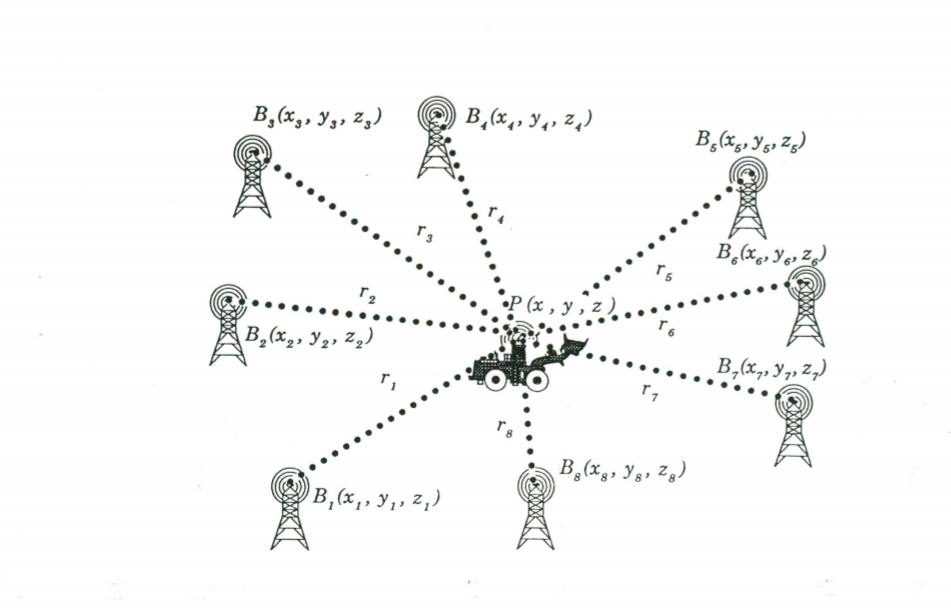
\includegraphics{dt1}}
    \caption{Разположение на получателите и предавателя в мина}
    \label{fig:mine}
\end{figure}

Разглежда се възможността за съствяне система от \textit{N} на брой нелинейни уравнения използвайки следната формула. Задачата се моделира като търсене на пресечни точки на N на брой сфери за всеки трансмитер.

\begin{equation}
    (x-x_i)^2 + (y-y_i)^2 +(z-z_i)^2=r_i^2
\end{equation}

Решението на гореспоменатата нелинейна система от уравнения се счита за неизползваема тъй като полученото уравнение е нелинейно и е от висока степен. Когато разстоянията, които са измерени са точни, а не са приблизителни, линезирането на системата от уравнения е удачно. Когато измерените разстояния са приблизителни е редно да се използват техниките \textit{линейни и нелинейни най-малки квадрати}.  